‫\فصل{نمونه اولیه معماری}
‫\زیرقسمت{معماری کلاینت سرور}
‫پس از بررسی موارد کاربرد و به دست آمدن دید کلی نسبت به نیازمندی‌های سیستم، به بررسی راه‌حل‌هایی برای معماری سیستم می‌پردازیم. رویکرد ما برای معماری جداکردن دغدغه‌ها برای به‌کارگیری تصمیمات و مکانیزم‌های لازم در مواجهه با ریسک‌های سیستم است. بنابراین در طول مسیر و برای ساختن معماری،  ابتدا مطابق تحلیل اولیه، زیرسیستم‌های تحلیل را به عنوان کامپوننت‌های اصلی سیستم در نظر می‌گیریم.
‫با جدا کردن دغدغه‌های مربوط به نمایش سیستم و منطق، می‌توان هم از پیچیدگی سیستم کاست و تقسیم کار را بین اعضا را بهتر انجام داد که بدین ترتیب به این تصمیم رسیدیم که از معماری کلاینت سرور به دو بخش اصلی سیستم استفاده کنیم.
‫
‫\شروع{شکل}[ht]
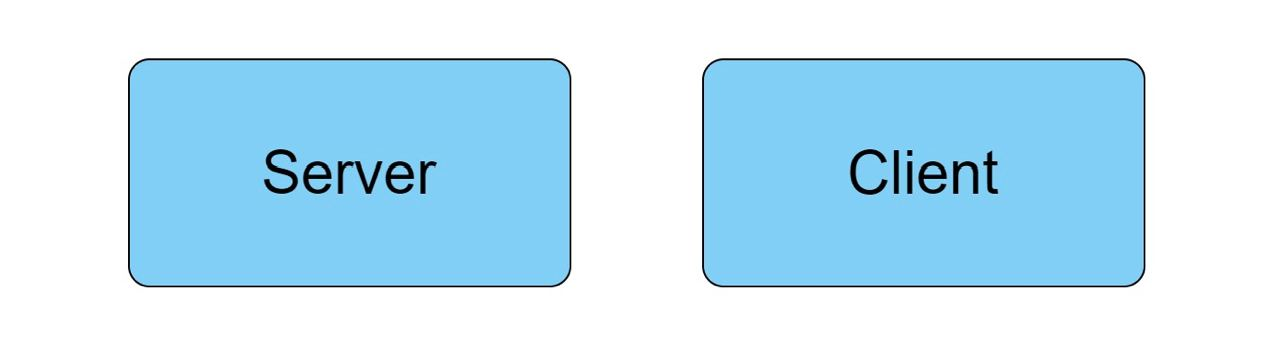
\includegraphics[scale=0.3]{figs/server_client.jpeg}
‫\شرح{معماری کلاینت سرور}
‫\برچسب{شکل:معماری کلاینت سرور}
‫\پایان{شکل}

‫\زیرقسمت{معماری زیرسیستم‌ها}
‫پس از آن برای ساختار داخلی سرور، برای اینکه به مدل‌های تحلیل و نیازمندی‌های مشتری نزدیک باشیم تا در صورت تغییرات بتوانیم آن را مدیریت کنیم، تلاش کردیم تا از همان زیرسیستم‌های اصلی به عنوان ساختار سطح بالا استفاده کنیم. به همین دلیل ساختار سطح بالای اولیه سیستم به شکل زیر خواهد بود:
‫
‫\شروع{شکل}[ht]
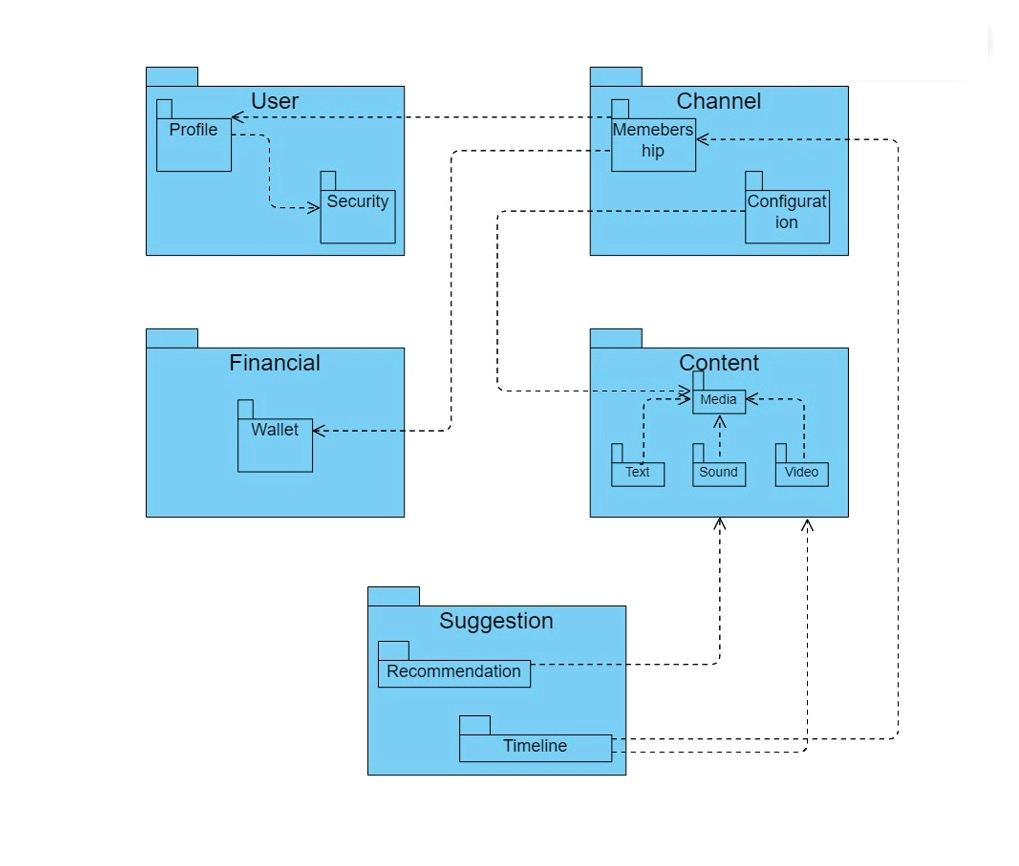
\includegraphics[scale=0.4]{figs/subsystem.jpg}
‫\شرح{نمودار بسته}
‫\برچسب{شکل:نمودار بسته}
‫\پایان{شکل}
‫
‫برای معماری سیستم از ساختار سطح بالای نمودار پکیج بالا و معادل آن استفاده می‌کنیم. در واقع سیستم را به تعدادی کامپوننت خواهیم شکست که هر کامپوننت مطابق معادل آن در نمودار پکیج خواهد بود که به دلیل ناکافی بودن جزئیات از آوردن آن صرف نظر شده است. در ادامه نیز هر کامپوننت به کامپوننت‌های کوچکتری خواهد شکست تا در نهایت تنها به فیچرهای‌ لازم و ریزدانه برسیم. همچنین مکانیزم‌های زیر برای مدیریت ریسک‌های موجود در پروژه اتخاذ شده است:
‫\شروع{شمارش}
‫\فقره استفاده از پروسه‌های اتمیک برای مدیریت پرداختی‌های کاربران که در کامپوننت financial لحاظ خواهد شد.
‫\فقره
‫نگهداری transactionهای سیستم به منظور بازیابی پرداخت‌ها در صورت بروز خطا که در کامپوننت financial لحاظ خواهد شد.
‫\پایان{شمارش}
‫
‫در هر کامپوننت یا زیرکامپوننت سیستم از یک ساختار سه‌سطحی استفاده می‌کنیم. هر کامپوننت، علاوه بر اینکه نیازمندی‌های لازم برای ارتباط با سایر بخش‌ها را از طریق نمای تعریف شده آن برآورده می‌سازد، بلکه مسئولیت ارتباطات مربوط به خود با کلاینت و پایگاه داده را نیز پیاده‌سازی می‌کند. این امر باعث یکپارچه‌سازی کامپوننت‌ها و نزدیک‌تر شدن به ساختار تحلیلی است.
‫\شروع{شکل}[ht]
‫\تنظیم‌ازوسط
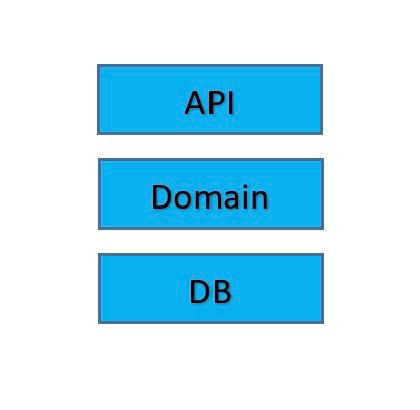
\includegraphics[scale=0.3]{figs/three_level.jpg}
‫\شرح{ساختار سه‌سطحی کامپوننت یا زیرکامپوننت‌ها}
‫\برچسب{شکل:ساختار سه‌سطحی کامپوننت یا زیرکامپوننت‌ها}
‫\پایان{شکل}
‫\زیرقسمت{نمودار استقرار}
‫برای مدیریت زیرساخت سیستم و ارتباط با سخت افزار نمودار زیر به عنوان یک دید از سطح بالا ترسیم گشته است:
‫\شروع{شکل}[ht]
‫\تنظیم‌ازوسط
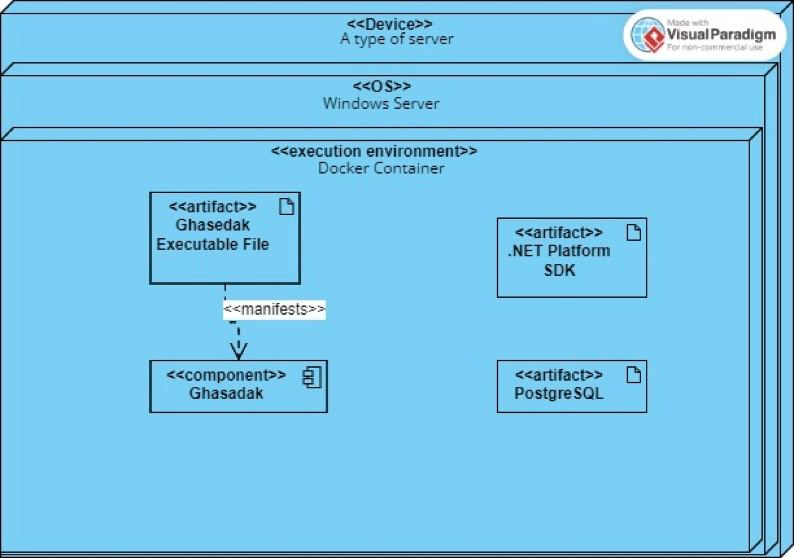
\includegraphics[scale=0.5]{figs/high_level.jpeg}
‫\شرح{نمودار استقرار}
‫\برچسب{شکل:نمودار استقرار}
‫\پایان{شکل}
‫
‫